\cleardoublepage\chapter{Related Work}\label{sec:related_work}\minitoc\vspace{.5cm}\index{SotA}

\section{Introduction}

% \begin{wrapfigure}{r}{0.2\textwidth}
%     \centering
%     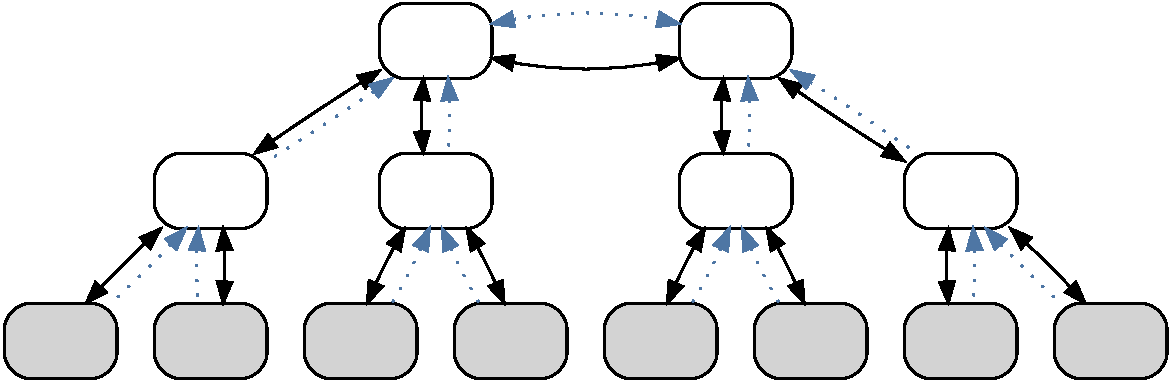
\includegraphics[width=0.2\textwidth]{resources/images/example3}
% \end{wrapfigure}

% \sidenote{Overview}
% \todomid{write}

Multipath is not a new concept. In this section we will visit notable existing multipath protocols, their characteristics and how is our concept differ from them.
Apart from that, we also discuss about future use case for our \ac{MTX} as well as the current solutions and 
technologies being used.
Finally, a quick dive into 5G system design with Data Plane as the main focus will explain our plan to demonstrate the multipath tunnel with \ac{gptu} protocol.

\section{Tunneling}\index{Tunneling}
% The term tunnel is borrowed from the real world where it described a confined physical transportation route that was built to direct traffic from A to B isolately from the terrain outside of the tunnel. 
% The physical tunnel is often dug deep down in the earth to bypass mountains, rivers, ocean channels ...
% In networking, from the application point of view, the tunnel is a direct network path to access another network from the network it is currently connected to.
% From the infrastructure perspective, the tunnel is an abstraction layer that omits the real traffic routing from the application and isolates the tunnel's traffic from public traffic, often by encapsulating application's data packet in tunnel's packet and extract the original data on the other end.
\todo{these following are my words, but do I need cite here?}
The concept of a tunnel draws inspiration from its real-world counterpart, which refers to a confined pathway constructed to direct transportation between two points, separate from the surrounding terrain. 
In the physical sense, tunnels are often excavated deep beneath the earth's surface to bypass obstacles like mountains, rivers, or ocean channels.
In the realm of networking, a tunnel can be perceived as a direct network pathway that enables access to another network from the network to which it is currently connected. 
From an infrastructure standpoint, a tunnel serves as an abstraction layer that abstracts the actual traffic routing from the application and isolates the tunnel's traffic from public network traffic. 
This is typically achieved by encapsulating the application's data packets within the tunnel's packets, and then extracting the original data at the other end of the tunnel.
Many tunnel protocols exist for different purposes: IPv4/IPv6 tunnels to enable compatibility between exclusive networks \cite{rfc4380_Teredo_ipv6_tunnel_udp}, Secure Shell (SSH) - tunnel for remote access and data transfer \cite{rfc4251_ssh_protocol}, and \ac{VPN} tunneling - used for access other network from another network. 
% \ac{VPN} is commonly used for accessing private network remotely (i.e, access university's private network from home network) and masking the network so traffic appears to be originated from VPN server (to bypass firewall or securely access network over untrusted connection like coffee shop's public WLAN)
\ac{VPN}s are frequently utilized to remotely access a private network, such as connecting to university's network from home. 
It also functions to conceal the origin of network traffic by making it appear as if it originates from the VPN server, which is useful for bypassing firewalls or restrictions applied by local network providers.
The traffic can also be encrypted to add an extra layer of protection while accessing networks over untrusted connections, like public WLANs found in coffee shops.

\ac{ovpnpage}

Some well known VPN protocols can be named wireguard, openvpn and ipsec. 

Our primary emphasis is on establishing a connection between two points, irrespective of the number of physical transportation links.


% \begin{figure}[H]
%     \centering
%     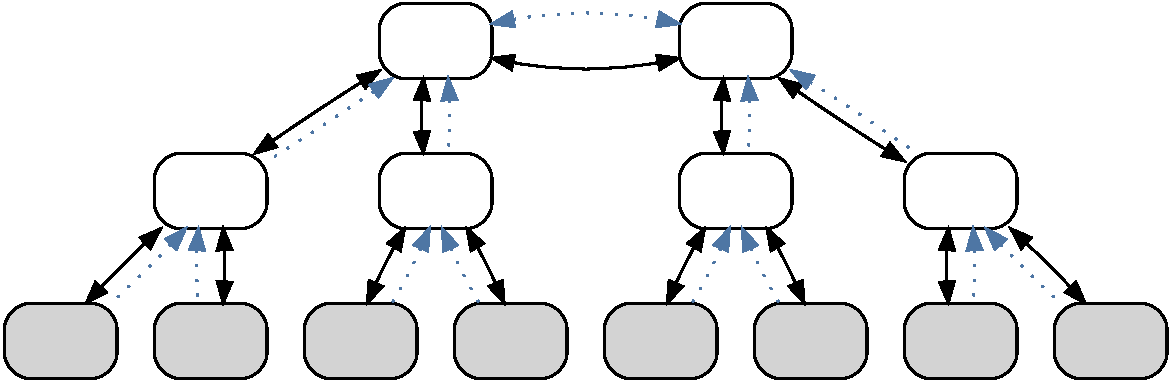
\includegraphics[width=.55\textwidth]{resources/images/example3}
%     \caption{Related area 1 within the structure of research}\label{fig:hourglass:ra1}
% \end{figure}

% \sidenote{Overview}
% \todomid{write about \Cref{fig:hourglass:ra1}}

% \sidenote{Focus}
% \todomid{write}

% \subsection{Specific Example 1}

% \sidenote{Definition}
% \todomid{write}

% \sidenote{Issues}
% \todomid{write}

% \subsection{Specific Example 2}

% \sidenote{Definition}
% \todomid{write}

% \sidenote{Implementations}
% \todomid{write}

% \sidenote{Research}
% \todomid{write}

% \sidenote{Standards}
% \todomid{write}

% \sidenote{Adoption}
% \todomid{write}

% \subsection{Specific Example 3}\index{Example 3}

% \sidenote{Transition}
% \todomid{write about \Cref{fig:sota:trans}}

% \begin{figure}
%     \centering
%     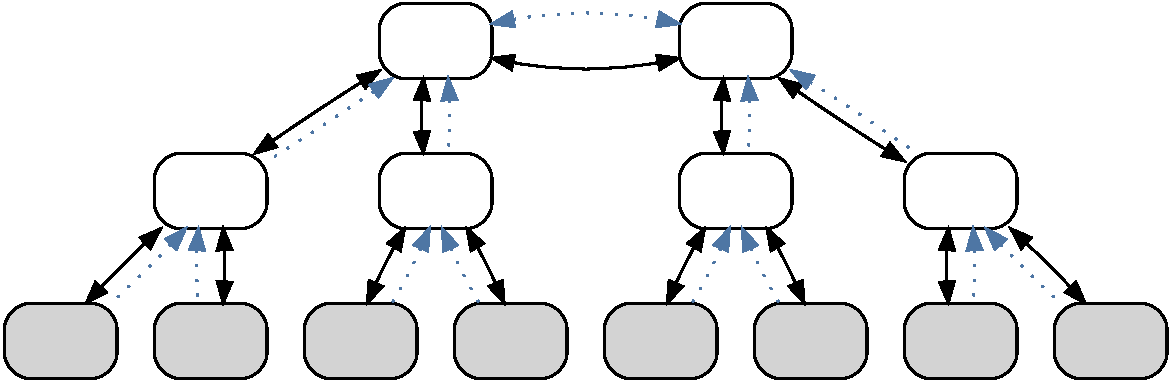
\includegraphics[width=.85\textwidth]{resources/images/example3}
%     \caption{Comparison of Example 2 and Example 3 (based on~\cite{li2002design})}\label{fig:sota:trans}
% \end{figure}

% \sidenote{Standards}
% \todomid{write}

% \sidenote{Extension}
% \todomid{write}

% \sidenote{Other Standards}
% \todomid{write}

% \sidenote{Something}
% \todomid{write}

% \sidenote{Something}
% \todomid{write}

% \sidenote{Something}
% \todomid{write}

% \sidenote{Something}
% \todomid{write}

% \sidenote{Something}
% \todomid{write}

% \sidenote{Something}
% \todomid{write}

% \section{Related Area 2}\index{Related Area 2}

% \sidenote{Overview}
% \todomid{write}

% \sidenote{Focus}
% \todomid{write about \Cref{fig:sota:ra2}}

% \begin{figure}[!hbtp]
%     \centering
%     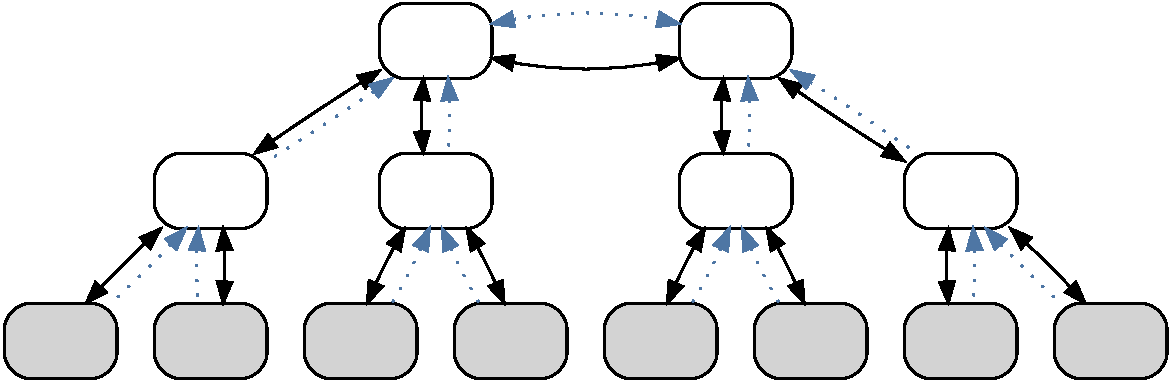
\includegraphics[width=1\textwidth]{resources/images/example3}
%     \caption{Related Area 2}\label{fig:sota:ra2}
% \end{figure}

% \sidenote{Something}
% \todomid{write}

% \subsection{Specific Example 1}

% \sidenote{Definition}
% \todomid{write}

% \sidenote{Issues}
% \todomid{write}

% \subsection{Specific Example 2}

% \sidenote{Definition}
% \todomid{write}

% \sidenote{Implementations}
% \todomid{write}

% \sidenote{Research}
% \todomid{write}

% \sidenote{Standards}
% \todomid{write}

% \sidenote{Adoption}
% \todomid{write}


% \section{Related Area 3}\index{Related Area 3}

% \sidenote{Overview}
% \todomid{write}

% \sidenote{Focus}
% \todomid{write about \Cref{fig:sota:ra3}}

% \begin{figure}[!hbtp]
%     \centering
%     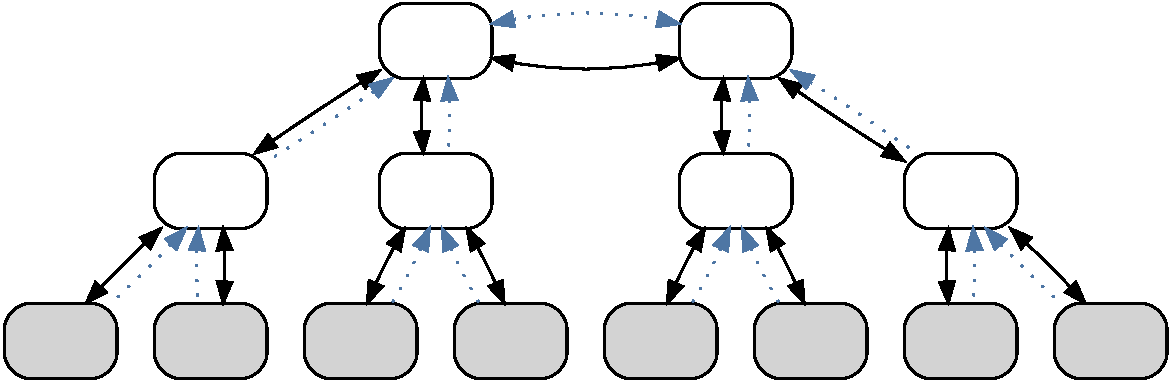
\includegraphics[width=1\textwidth]{resources/images/example3}
%     \caption{Related Area 3}\label{fig:sota:ra3}
% \end{figure}

% \sidenote{Something}
% \todomid{write}

% \subsection{Specific Example 1}

% \sidenote{Definition}
% \todomid{write}

% \sidenote{Issues}
% \todomid{write}

% \subsection{Specific Example 2}

% \sidenote{Definition}
% \todomid{write}

% \sidenote{Implementations}
% \todomid{write}

% \sidenote{Research}
% \todomid{write}

% \sidenote{Standards}
% \todomid{write}

% \sidenote{Adoption}
% \todomid{write}

% \section{Conclusion}

% \sidenote{Summary}
% \todomid{write}

% \sidenote{Takeaway 1}
% \todomid{write}

% \sidenote{Takeaway 2}
% \todomid{write}

% \sidenote{Takeaway 3}
% \todomid{write}

% \sidenote{Next chapter}
% \todomid{write}
